\documentclass{beamer}
\usetheme{default}
\usepackage{graphicx}
\usepackage{hyperref}
\usepackage{amsmath}
\title{
    Fluid Simulation with\\
    Smoothed Particle Hydrodynamics(SPH) method\\
    accelerated with Compute Shaders\\
    ${\quad}$\\
    \small{Final project for the practical course in Computergrafik 2016}
}
\author{Fabian Klemp\\
    \small{FH Aachen}\\
}
\date{30 June, 2016}
\setbeamertemplate{bibliography item}{}
\setbeamertemplate{footline}{\hspace*{\fill}\insertframenumber/\inserttotalframenumber\hspace*{\fill}\vskip15pt}
\usenavigationsymbolstemplate{}
\begin{document}
{
\setbeamertemplate{footline}{}
\begin{frame}[noframenumbering]
    \maketitle
\end{frame}
}
\begin{frame}
    \frametitle{Table of Contents}
    \tableofcontents
\end{frame}

\section{Introduction}
\begin{frame}
    \frametitle{Fluids}
    \begin{itemize}
        \item Liquids, e.g. water
        \item Gasses, e.g. air
        \item Plasmas
    \end{itemize}
\end{frame}
\begin{frame}
    \frametitle{Introduction/Motivation}
    \begin{center}
        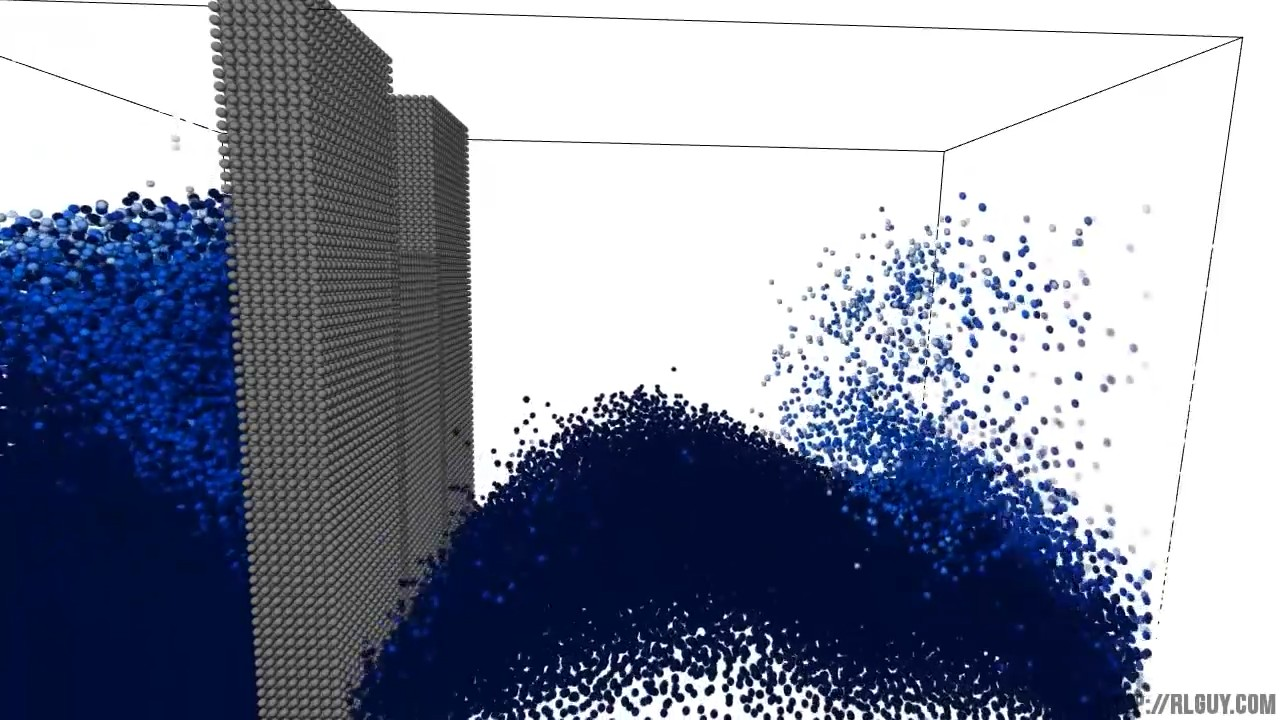
\includegraphics[width=10cm]{introduction.jpg}
    \end{center}
    \begin{flushright}
        source: \href{https://youtu.be/iHACAlfYeiQ}{https://youtu.be/iHACAlfYeiQ}
    \end{flushright}
\end{frame}


\section{Formula}
\begin{frame}
    \frametitle{Navier-Stokes-Equations}
    Equations which describe the motion of viscous fluids.\\
    $\qquad$\\
    We use the Navier-Stokes-Equations for incompressible fluids with constant density:\\
    \begin{align*}
        \frac{\partial\boldsymbol{v}}{\partial t} + (\boldsymbol{v} \cdot \nabla )\boldsymbol{v} = 
        \boldsymbol{g} - \nabla \frac{\boldsymbol{p}}{\rho} + \frac{\mu}{\rho}\nabla^2\boldsymbol{v} 
    \end{align*}
    where $\boldsymbol{v}$ is the velocity, $\boldsymbol{g}$ is the gravity,
    $\boldsymbol{p}$ is the pressure and $\rho$ and $\mu$ are the material
    properties density and dynamic viscosity.
\end{frame}

\begin{frame}
    \frametitle{Smoothed Particle Hydrodynamics}
    Physical property $\Phi_i$ at position $r_i$ is computed in a sphere with radius $h$:
    \begin{align*}
        \Phi_i = \sum_j m_j W(h, \boldsymbol{r_i} - \boldsymbol{r_j})
    \end{align*}
    $W$ is the weighting function which sums to $1$ over radius $h$ and drops to $0$ outside of $h$.
\end{frame}

\begin{frame}
    \frametitle{Smoothed Particle Hydrodynamics}
    \begin{align*}
        \rho_i &\approx \sum_j m_j \frac{315}{64\pi h^9} \big(h^2-\lVert \boldsymbol{r_i} - \boldsymbol{r_j} \rVert^2\big)^3\\
        %
        p_i &= \rho_i - \rho_0\\
        %
        \frac{dv_i}{dt} &= \boldsymbol{g} -  \frac{\nabla\boldsymbol{p_i}}{\rho_i} + \frac{\mu}{\rho_i}\nabla^2\boldsymbol{v_i}\\
        %
        \frac{\nabla\boldsymbol{p_i}}{\rho_i} &\approx \sum_j m_j \bigg( \frac{\boldsymbol{p_i}}{\rho_i^2} + \frac{\boldsymbol{p_j}}{\rho_j^2}\bigg) 
        \frac{-45}{\pi h^6} \big(h-\lVert\boldsymbol{r_i} - \boldsymbol{r_j}\rVert\big) \frac{\boldsymbol{r_i} - \boldsymbol{r_j}}{\lVert \boldsymbol{r_i} - \boldsymbol{r_j}\rVert}\\
        %
        \frac{\mu}{\rho_i}\nabla^2\boldsymbol{v_i} &\approx \frac{\mu}{\rho_i}\sum_j m_j \bigg(\frac{\boldsymbol{v_j} - \boldsymbol{v_i}}{\rho_j}\bigg)
        \frac{45}{\pi h^6}\big(h - \lVert\boldsymbol{r_i} - \boldsymbol{r_j}\rVert\big)\\
        %
        \frac{dv_i}{dt} &= \boldsymbol{g} -  \frac{\nabla\boldsymbol{p_i}}{\rho_i} + \frac{\mu}{\rho_i}\nabla^2\boldsymbol{v_i}
    \end{align*}
\end{frame}



\begin{frame}
    \frametitle{Evaluation}
    Content:
    \begin{itemize}
        \item very few Parameters
        \item no assumptions about the data, but still meaningfull results
        \item comparable performance to established methods
        \item Parameter choices still existent:
            \begin{itemize}
                \item motif\_length
                \item background\_noise
                \item conversion from audio data to spectogram
                \item MPEG encoding
            \end{itemize}
    \end{itemize}
\end{frame}

\begin{frame}
    \frametitle{Evaluation}
    Presentation:
    \begin{itemize}
        \item good Visualization with spectograms and graphs
        \item Pseudo Code is a bit confusing
        \item Code not directly accessible, unlike stated in the paper
        \item Enclosed code is in a bad state, bad documented
    \end{itemize}
\end{frame}

\begin{frame}
    \frametitle{Thank you for your attention}
    \begin{center}
        Any Questions?\\
        Feedback?
    \end{center}
    
\end{frame}


\begin{frame}
    \frametitle{Sources}
    \nocite{haoparameter}
    \nocite{campana2010compression}
    \nocite{keogh2012monitoring}
    \bibliographystyle{unsrt}
    \bibliography{sources}
\end{frame}

\end{document}
